%Täänne on kerätty tehtävät muiden kirjojen käyttämässä tehtävä-ympäristössä
%
%ESIMERKKI
%
%
%
%\begin{tehtava}
%    
%   \begin{vastaus}
%   \end{vastaus}
%    
%\end{tehtava}
%
%
%\begin{tehtava}
%    
%    \begin{alakohdat}
%        \alakohta{}
%        \alakohta{}
%        \alakohta{}
%    \end{alakohdat}
%
%    \begin{vastaus}
%        \begin{alakohdat}
%            \alakohta{}
%            \alakohta{}
%            \alakohta{}
%        \end{alakohdat}
%    \end{vastaus}
%    
%\end{tehtava}

%luku logiikka ja päättely


%Harj.Tehtävät Luku 1, Vastausten tekijä Valtteri Vistiaho 9.11.2013
\begin{tehtava}
    Onko päättely loogisesti pätevä? Perustele.
    \begin{alakohdat}
        \alakohta{Kaikki ihmiset ovat kuolevaisia. Lasse-kissa on kuolevainen. Siis Lasse-kissa on ihminen.}
        \alakohta{Kaikki koirat osaavat haukkua. Halli on koira. Siis Halli osaa haukkua.}
    \end{alakohdat}

    \begin{vastaus}
        \begin{alakohdat}
            \alakohta{Ei}
            \alakohta{On}
        \end{alakohdat}
    \end{vastaus}
    
\end{tehtava}

\begin{tehtava}
    Ovatko seuraavat päättelyt loogisesti päteviä? Perustele.
    \begin{alakohdat}
        \alakohta{\kolmepaattely{Kaikki tetraedrit ovat pyramideja.}{Jotkut kartiot ovat tetraedrejä.}
                {Jotkut kartiot ovat pyramideja.}}
        \alakohta{\kolmepaattely{Kaikki sylinterit ovat lieriöitä.}{Mikään lieriö ei ole kartio.}
                {Jotkut sylinterit ovat kartioita.}}
        \alakohta{\kolmepaattely{Luku $345$ päättyy numeroon $5$.}{Nollaan päättyvä luku on viidellä jaollinen.}
                {Luku $345$ on viidellä jaollinen.}}	        
    \end{alakohdat}

    \begin{vastaus}
        \begin{alakohdat}
            \alakohta{On}
            \alakohta{Ei}
            \alakohta{Ei}
        \end{alakohdat}
    \end{vastaus}
    
\end{tehtava}

\begin{tehtava}
    Onko seuraava päättely loogisesti pätevä? Perustele.
    \begin{alakohdat}
        \alakohta{Jos ulkona on pakkanen, menen hiihtämään. Ulkona ei ole pakkanen. Siis en mene hiihtämään.}
        \alakohta{Jos ulkona on pakkanen, menen hiihtämään. En mene hiihtämään. Siis ulkona ei ole pakkanen.}
        \alakohta{Jos tiedän nukkuvani, niin nukun. Jos tiedän nukkuvani, niin en nuku. Siis en tiedä nukkuvani.}
    \end{alakohdat}

    \begin{vastaus}
        \begin{alakohdat}
            \alakohta{On}
            \alakohta{Ei}
            \alakohta{Ei, ???????????????} %En ole täysin varma vastauksesta
        \end{alakohdat}
    \end{vastaus}
    
\end{tehtava}

\begin{tehtava}
    Tutkitaan polynomia
        \[ P(x) = x^5 -10x^4+35x^3 -50 x^2 +25x. \]
    \begin{alakohdat}
        \alakohta{Laske $P(0)$, $P(1)$, $P(2)$, $P(3)$ ja $P(4)$.}
        \alakohta{Mitä voit sanoa luvuista $P(n)$, kun $n$ on luonnollinen luku?}
        \alakohta{Testaa päätelmääsi kokeilemalla myös muilla luonnollisilla luvuilla esimerkiksi laskinta käyttäen.}
    \end{alakohdat}

    \begin{vastaus}
        \begin{alakohdat}
            \alakohta{$P(0)=0$, $P(1)=1$, $P(2)=2$, $P(3)=3$, $P(4)=4$}
            \alakohta{$P(n)=n$}
            \alakohta{$P(5)=125$, päätelmä ei päde.}
        \end{alakohdat}
    \end{vastaus}
    
\end{tehtava}

\begin{tehtava}
    Arkiajattelussa käytetään usein ajattelumalleja, jotka eivät ole loogisesti perusteltavissa.
        Mikä virhe on seuraavissa päätelmissä?
    \begin{alakohdat}
        \alakohta{Ilta-Sanomien kyselyssä $66~\%$ vastaajista uskoo maan ulkopuoliseen elämään.
                Maan ulkopuolista elämää on olemassa.}
        \alakohta{The Sunday Times -lehden haastattelussa kuuluisa tiedemies Stephen Hawking
                totesi pitävänsä lähes varmana, että avaruudessa on maan ulkopuolista älykästä elämää.
                Maan ulkopuolista elämää on olemassa.}
        \alakohta{Tiedemiehistä 90~\% väittää, että nykyinen ilmastonmuutos on ihmisen aiheuttamaa
                eikä johdu maapallon lämpötilan luontaisesta jaksollisuudesta.
                Siis nykyinen ilmastonmuutos on ihmisen aiheuttamaa.}
        \alakohta{Televisiouutisissa kerrottiin, että toisen maailmansodan aikainen holokausti oli
                vain liittoutuneiden propagandaa.
                Siis holokaustia ei tapahtunut toisen maailmansodan aikana.}
    \end{alakohdat}

    \begin{vastaus}
        \begin{alakohdat}
            \alakohta{Johtopäätös vedetty vastaajien uskomuksesta.}
            \alakohta{Johtopäätös vedetty Stephen Hawkingin uskomuksesta.}
            \alakohta{Johtopäätös perustuu tiedemiehien väitteisiin, joista ei ole varmaa totuutta.}
            \alakohta{Johtopäätös perustuu televisiouutisen väitteeseen, josta ei ole selviä todisteita.}
        \end{alakohdat}
    \end{vastaus}
    
\end{tehtava}

\begin{tehtava}
    Ovatko seuraavat päättelyt loogisesti päteviä? Perustele.
    \begin{alakohdat}
        \alakohta{\kolmepaattely{Kaikilla $x$ toteutuu $y$.}{Joillakin $z$ toteutuu $x$.}{Joillakin $z$ toteutuu $y$.}}
        \alakohta{\kolmepaattely{Kaikilla $A$ toteutuu $B$.}{$C$ toteuttaa $B$:n.}{$C$ toteuttaa $A$:n.}}
        \alakohta{\kolmepaattely{Kaikilla $A$ toteutuu $B$.}{Millään $C$ ei toteudu $B$.}{Millään $C$ ei toteudu $A$.}}
    \end{alakohdat}

    \begin{vastaus}
        \begin{alakohdat}
            \alakohta{On}
            \alakohta{Ei. Jos A toteuttaa B:n, B ei välttämättä toteuta A:ta.}
            \alakohta{Ei, ?????????????} %En ole täysin varma vastauksesta
        \end{alakohdat}
    \end{vastaus}
    
\end{tehtava}
%Kotitehtävät Luku 1, Vastausten tekijä Valtteri Vistiaho 9.11.2013
\begin{tehtava}
    Ovatko seuraavat päättelyt päteviä? Perustele.
    \begin{alakohdat}
        \alakohta{\kolmepaattely{Kaikki kissat osaavat kehrätä.}{Tämä eläin osaa kehrätä.}{Tämä eläin on kissa.}}
        \alakohta{\kolmepaattely{Kukaan laiska opiskelija ei selviä kokeesta.}
                {On opiskelijoita, jotka selviävät kokeesta.}{On opiskelijoita, jotka eivät ole laiskoja.}}
    \end{alakohdat}

    \begin{vastaus}
        \begin{alakohdat}
            \alakohta{Ei}
            \alakohta{On}
        \end{alakohdat}
    \end{vastaus}
    
\end{tehtava}

\begin{tehtava}
    Ovatko seuraavat päättelyt päteviä? Perustele.
    \begin{alakohdat}
        \alakohta{\kolmepaattely{Neljäkkään lävistäjät ovat kohtisuorassa toisiaan vastaan.}
                {Neljäkäs on suunnikas.}{Suunnikkaan lävistäjät ovat kohtisuorassa toisiaan vastaan.}}
        \alakohta{\kolmepaattely{Kaikki suorakulmiot ovat suunnikkaita.}{Jotkut nelikulmiot ovat suorakulmioita.}
                {Jotkut nelikulmiot ovat suunnikkaita.}}
        \alakohta{\kolmepaattely{Kolmio $ABC$ on tasakylkinen.}{Tasasivuiset kolmiot ovat tasakylkisiä.}
                {Kolmio $ABC$ on tasasivuinen.}}
    \end{alakohdat}

    \begin{vastaus}
        \begin{alakohdat}
            \alakohta{Ei}
            \alakohta{On}
            \alakohta{Ei}
        \end{alakohdat}
    \end{vastaus}
    
\end{tehtava}

\begin{tehtava}
    Ovatko seuraavat päättelyt päteviä? Perustele.
    \begin{alakohdat}
        \alakohta{\kaksipaattely{Kaikki lammasfarmin lampaat ovat joko mustia tai valkoisia.}
                {Kaikki lampaat ovat mustia tai valkoisia.}}
        \alakohta{\neljapaattely{Tavallisessa korttipakassa kortti on aina joko pata,\\& risti, hertta tai ruutu.}
                {Pata- ja risti-kortit ovat mustia.}{Hertta- ja ruutu-kortit ovat punaisia.}
                {Kaikki tavallisten korttipakkojen kortit ovat\\ & joko mustia tai punaisia.}}
    \end{alakohdat}

    \begin{vastaus}
        \begin{alakohdat}
            \alakohta{Ei}
            \alakohta{On}
        \end{alakohdat}
    \end{vastaus}
    
\end{tehtava}

\begin{tehtava}
    Jäämaa on kokonaan Merimaan itäpuolella.
        Kummallakin on etelärajaa Aurinkomaan kanssa.
        Merimaalla ja Aurinkomaalla on länsiraja Lumimaan kanssa.
        Kukkamaa on kokonaan Jäämaan ja Aurinkomaan itäpuolella.
    \begin{alakohdat}
        \alakohta{Onko Merimaalla ja Kukkamaalla yhteistä rajaa?}
        \alakohta{Voiko Lumimaalla ja Kukkamaalla olla yhteistä rajaa?}
    \end{alakohdat}

    \begin{vastaus}
        \begin{alakohdat}
            \alakohta{Ei}
            \alakohta{Ei, ?????????????} %En ole täysin varma vastauksesta
        \end{alakohdat}
    \end{vastaus}
    
\end{tehtava}

\begin{tehtava}
    Ovatko seuraavat päättelyt päteviä? Perustele.
    \begin{alakohdat}
        \alakohta{\kolmepaattely{Millään $x$ ei toteudu $y$.}{Kaikilla $z$ toteutuu $x$.}{Millään $z$ ei toteudu $y$.}}
        \alakohta{\kolmepaattely{Kaikilla $A$ toteutuu $B$.}{Joillakin $C$ toteutuu $B$.}{Joillakin $A$ toteutuu $C$.}}
    \end{alakohdat}

    \begin{vastaus}
        \begin{alakohdat}
            \alakohta{On}
            \alakohta{Ei}
        \end{alakohdat}
    \end{vastaus}
    
\end{tehtava}
%Harj. Tehtävät Luku 2, Vastausten tekijä Valtteri Vistiaho 9.11.2013
\begin{tehtava}
    Onko lause atomilause?
    \begin{alakohdat}
        \alakohta{Tampere on Pirkanmaalla.}
        \alakohta{Kajaani on Suomen pääkaupunki.}
        \alakohta{Hattu pois päästä!}
        \alakohta{On olemassa suurin alkuluku.}
        \alakohta{Onko avaruudessa elämää?}
        \alakohta{$5 + 12 = 18$.}
    \end{alakohdat}

    \begin{vastaus}
        \begin{alakohdat}
            \alakohta{On}
            \alakohta{On}
            \alakohta{Ei}
            \alakohta{On}
            \alakohta{Ei, ?????????} %En ole täysin varma vastauksesta
            \alakohta{On, ?????????} %En ole täysin varma vastauksesta
        \end{alakohdat}
    \end{vastaus}
    
\end{tehtava}

\begin{tehtava}
    Kirjoita lauseen negaatio.
    \begin{alakohdat}
        \alakohta{Tänään on maanantai.}
        \alakohta{$2+3=5$.}
        \alakohta{Luku on negatiivinen.}
        \alakohta{Ainakin yhdellä ryhmämme opiskelijalla on ruskeat silmät.}
        \alakohta{Kymmenessä sivussa tekstiä on vähintään seitsemän virhettä.}
        \alakohta{Kesä Välimerellä on kuuma ja aurinkoinen.}
    \end{alakohdat}

    \begin{vastaus}
        \begin{alakohdat}
            \alakohta{Tänään ei ole maanantai.}
            \alakohta{$2+3\neq5$}
            \alakohta{Luku on positiivinen.}
            \alakohta{Ainakin yhdellä ryhmämme opiskelijalla ei ole ruskeita silmiä.}
            \alakohta{Kymmenessä sivussa tekstiä on vähintään seitsemän virhettä.}
            \alakohta{Kesä Välimerellä on kylmä ja pilvinen.}
        \end{alakohdat}
    \end{vastaus}
    
\end{tehtava}

\begin{tehtava}
    Olkoot lause $A$: ''veikkasin lottorivin'' ja lause $B$: ''voitin miljoona euroa''. Kirjoita suomen kielellä lauseet
    \begin{alakohdat}
        \alakohta{$\lnot A$,}
        \alakohta{$A\lor B$,}
        \alakohta{$A\land B$,}
        \alakohta{$A\land \lnot B$,}
        \alakohta{$\lnot A\lor (A\land B)$,}
        \alakohta{$\lnot A\land \lnot B$.}
    \end{alakohdat}

    \begin{vastaus}
        \begin{alakohdat}
            \alakohta{En veikannut lottoriviä.}
            \alakohta{Veikkasin lottorivin tai voitin miljoona euroa.}
            \alakohta{Veikkasin lottorivin ja voitin miljoona euroa.}
            \alakohta{Veikkasin lottorivin ja en voittanut miljoonaa euroa.}
            \alakohta{En veikannut lottoriviä tai veikkasin lottorivin ja voitin miljoona euroa.}
            \alakohta{En veikannut lottoriviä enkä voittanut miljoonaa euroa.}
        \end{alakohdat}
    \end{vastaus}
    
\end{tehtava}

\begin{tehtava}
    Olkoot lause $A$: ''on kaunis kesäpäivä'',  lause $B$: ''lokit kirkuvat'' ja lause $C$: ''kävelen rannalla''. Kirjoita suomen kielellä lauseet
    \begin{alakohdat}
        \alakohta{$\lnot A\lor B$,}
        \alakohta{$A\land B \land C$,}
        \alakohta{$\lnot(A\land C)$,}
        \alakohta{$(A\land C)\lor (B\land
\lnot C)$.}
    \end{alakohdat}

    \begin{vastaus}
        \begin{alakohdat}
            \alakohta{Ei ole kaunis kesäpäivä tai lokit kirkuvat.}
            \alakohta{On kaunis kesäpäivä, lokit kirkuvat ja kävelen rannalla.}
            \alakohta{Ei ole totta, että on kaunis kesäpäivä ja kävelen rannalla.}
            \alakohta{On kaunis kesäpäivä ja kävelen rannalla tai lokit kirkuvat ja en kävele rannalla.}
        \end{alakohdat}
    \end{vastaus}
    
\end{tehtava}

\begin{tehtava}
    Olkoot $A$: ''on pilvistä'' ja $B$: ''sataa
lunta''. Formalisoi seuraavat lauseet eli kirjoita ne
lauseiden $A$ ja $B$ sekä konnektiivien $\lnot$, $\land$
ja $\lor$ avulla.
    \begin{alakohdat}
        \alakohta{On pilvistä ja sataa lunta.}
        \alakohta{On pilvistä, mutta ei sada lunta.}
        \alakohta{Ei ole pilvistä eikä sada lunta.}
        \alakohta{On pilvistä tai sataa lunta.}
        \alakohta{On pilvistä ja sataa lunta tai ei ole pilvistä
eikä sada lunta.}
    \end{alakohdat}

    \begin{vastaus}
        \begin{alakohdat}
            \alakohta{$A\land B$}
            \alakohta{$A\land \lnot B$}
            \alakohta{$\lnot A \land \lnot B$}
            \alakohta{$A \lor B$}
            \alakohta{$(A\land B)\lor \lnot A\land \lnot B$}
        \end{alakohdat}
    \end{vastaus}
    
\end{tehtava}

\begin{tehtava}
    Formalisoi lauseet:
    \begin{alakohdat}
        \alakohta{Mustikat polun varrella ovat kypsiä tai
alueella ei ole nähty karhuja.}
        \alakohta{Ei ole totta, että mustikat polun varrella ovat
kypsiä tai alueella on nähty karhuja.}
        \alakohta{Mustikat polun varrella ovat kypsiä, mutta
alueella ei ole nähty karhuja, tai sitten mustikat eivät
ole kypsiä ja alueella on nähty karhuja.}
        \alakohta{Karhuja ei ole nähty alueella ja polulla
vaeltaminen on turvallista, mutta mustikat ovat kypsiä.}
    \end{alakohdat}

    \begin{vastaus}
    Olkoot $A$: ''Mustikat polun varrella ovat kypsiä.'', $B$: ''Alueella on nähty karhuja.'' ja $C$: ''Polulla vaeltaminen on turvallista.''
        \begin{alakohdat}
            \alakohta{$A \lor \lnot B$}
            \alakohta{$\lnot(A\lor B)$}
            \alakohta{$(A\land \lnot B)\lor(\lnot A\land B)$}
            \alakohta{$\lnot B\land C\land A)$}
        \end{alakohdat}
    \end{vastaus}
    
\end{tehtava}

\begin{tehtava}
    
    \begin{alakohdat}
        \alakohta{Laadi totuustaulu lauseelle $\lnot A\lor \lnot
B$. Millä atomilauseiden $A$ ja $B$ totuusarvoilla lause
on tosi?}
        \alakohta{Laadi totuustaulu lauseelle $\lnot(A\land B)$.
Millä atomilauseiden $A$ ja $B$ totuusarvoilla lause on
tosi? Vertaa a-kohdan tulokseen.}
        \alakohta{Keksi atomilauseet $A$ ja $B$ ja ilmaise a- ja
b-kohtien lauseet suomen kielellä.}
    \end{alakohdat}

    \begin{vastaus}
        \begin{alakohdat}
            \alakohta{
            \begin{center}
		    \begin{tabular}{|c|c|c|c|c|}\hline
		    $A$ & $B$ & $\lnot A$ & $\lnot B$ & $\lnot A\lor \lnot B$\\ \hline
		    $1$ & $1$ & $0$ & $0$ & $0$  \\ %\hline
		    $1$ & $0$ & $0$ & $1$ & $1$  \\
		    $0$ & $1$ & $1$ & $0$ & $1$  \\
		    $0$ & $0$ & $1$ & $1$ & $1$  \\ \hline
\end{tabular}
\end{center}}
            \alakohta{
            \begin{center}
		    \begin{tabular}{|c|c|c|}\hline
		    $A$ & $B$ & $\lnot(A\land B)$\\ \hline
		    $1$ & $1$ & $0$  \\ %\hline
		    $1$ & $0$ & $1$  \\
		    $0$ & $1$ & $1$  \\
		    $0$ & $0$ & $1$  \\ \hline
\end{tabular}
\end{center}}
            \alakohta{Ei sada tai ei tuule.\newline Ei ole totta, että sataa ja tuulee.}
        \end{alakohdat}
    \end{vastaus}
    
\end{tehtava}

\begin{tehtava}
    Laadi totuustaulu lauseelle $(A\land B)\lor \lnot (B\lor C)$.

    \begin{vastaus}
        \begin{center}
		    \begin{tabular}{|c|c|c|c|c|c|c|}\hline
		    $A$ & $B$ & $C$ & $B\lor C$ & $A\land B$ & $\lnot (B\lor C)$ & $(A\land B)\lor \lnot (B\lor C)$\\ \hline
		    $1$ & $1$ & $1$ & $1$ & $1$ & $0$ & $1$  \\ %\hline
		    $1$ & $1$ & $0$ & $1$ & $1$ & $0$ & $1$  \\
		    $1$ & $0$ & $1$ & $1$ & $0$ & $0$ & $0$  \\
		    $1$ & $0$ & $0$ & $0$ & $0$ & $1$ & $1$  \\
		    $0$ & $1$ & $1$ & $1$ & $0$ & $0$ & $0$  \\
		    $0$ & $1$ & $0$ & $1$ & $0$ & $0$ & $0$  \\
		    $0$ & $0$ & $1$ & $1$ & $0$ & $0$ & $0$  \\
		    $0$ & $0$ & $0$ & $0$ & $0$ & $1$ & $1$  \\ \hline
\end{tabular}
\end{center}
    \end{vastaus}
    
\end{tehtava}

\begin{tehtava}
    Olkoot atomilauseet $A$: ''$x < -1$'', $B$: ''$x > 1$''  ja $C$: ''$x = 1$''. Formalisoi  lauseet
    \begin{alakohdat}
        \alakohta{$x\neq 1$,}
        \alakohta{$x \ge 1$,}
        \alakohta{$x \ge -1$,}
        \alakohta{$x < 1$,}
        \alakohta{$-1 \le x \le  1$,}
        \alakohta{$x <  -1$ tai $x  \ge 1$.}
    \end{alakohdat}

    \begin{vastaus}
        \begin{alakohdat}
            \alakohta{$\lnot C$}
            \alakohta{$B\lor C$}
            \alakohta{$\lnot A$}
            \alakohta{$\lnot(B\lor C)$}
            \alakohta{$\lnot(A\land B$}
            \alakohta{$A\lor (B\lor C)$}
        \end{alakohdat}
    \end{vastaus}
    
\end{tehtava}

\begin{tehtava}
    Saarella asuu haltijoita ja menninkäisiä. Turisti tapasi kaksi saarelaista, Hipsun ja Vipsun. Hipsu sanoi: ''Hillat ovat kypsiä ja kalaonni on suotuisa, tai sitten hillat eivät ole kypsiä tai kalaonni ei ole suotuisa.'' Vipsu väitti: ''Hillat ovat kypsiä ja kalaonni on suotuisa, mutta hillat eivät ole kypsiä tai kalaonni ei ole suotuisa.'' Tutki totuustaulun avulla Hipsun ja Vipsun väitteiden totuusarvoja. Mitä voidaan päätellä totuustaulun avulla, kun tiedetään, että saaren asukkaista haltijat valehtelevat aina ja menninkäiset puhuvat aina totta? Saiko vierailija käyttökelpoista tietoa marjasadosta tai kalaonnesta?

    \begin{vastaus}
    Olkoot $A$: ''Hillat ovat kypsiä.'' ja $B$: ''Kalaonni on suotuisa.''
    \begin{center}
		    \begin{tabular}{|c|c|c|c|c|c|c|c|}\hline
		    $A$ & $B$ & $\lnot A$ & $\lnot B$ & $A\land B$ & 
		         $\lnot A\lor \lnot B$ & $(A \land B)\lor(\lnot A\lor \lnot B)$ & $(A\land B)\land(\lnot A\lor \lnot B)$ \\ \hline
		    $1$ & $1$ & $0$ & $0$ & $1$ & $0$ & $1$ & $0$  \\ %\hline
		    $1$ & $0$ & $0$ & $1$ & $0$ & $1$ & $1$ & $0$  \\
		    $0$ & $1$ & $1$ & $0$ & $0$ & $1$ & $1$ & $0$  \\
		    $0$ & $0$ & $1$ & $1$ & $0$ & $1$ & $1$ & $0$  \\ \hline
\end{tabular}
\end{center}
	??????????????????????????????????????????????????????????????? %Tehtävä on melko epäselvä, mahdollisesti monta eri tulkintaa.
    \end{vastaus}
    
\end{tehtava}

\begin{tehtava}
    Loogisilla piireillä suoritetaan digitaalisissa laitteissa erilaisia loogisia operaatioita. Loogisen piirin toimintaa voidaan kuvata esimerkiksi seuraavalla kaaviolla.

\medskip

\begin{center}
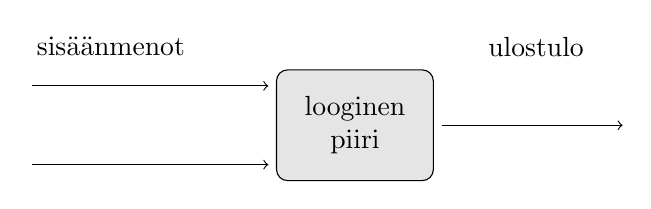
\begin{tikzpicture}
\node [rectangle, draw, fill=gray!20, text width=5em, text centered, rounded corners, minimum height=4em] at (4.1,1) {looginen piiri};
\draw [->] (0,0.5) -- (3,0.5);
\draw [->] (0,1.5) -- (3,1.5);
\draw [->] (5.2,1) -- (7.5,1);


\node at (1,2) {sisäänmenot};
\node at (6.4,2) {ulostulo};
\end{tikzpicture}
\end{center}

\medskip

Loogisella piirillä on yksi tai useampi sisäänmeno ja
yksi tai useampi ulostulo. Tämän kirjan esimerkeissä ja
tehtävissä käsitellään vain yhden ulostulon piirejä.
Sisäänmenojen ja ulostulon signaalin arvo
voi olla 1 tai 0. Edellisessä tapauksessa johtimessa on
jännite, jälkimmäisessä tapauksessa ei ole.

Loogiset piirit kootaan loogisista porteista. Seuraavassa
taulukossa on lueteltu loogiset portit, niiden toiminta
ja toimintaa vastaava looginen konnektiivi.

%\newpage

\small

\begin{center}
\begin{tabular}{|>{\centering}m{1.5cm}|>{\raggedright}m{3.8cm}|c|>{\centering\arraybackslash}m{2cm}|}
\hline
Looginen portti & \centering Toiminta & Piirrosmerkki & Looginen konnektiivi \\
% \begin{tabular}{c}
% %Toimintaa \\
% %	vastaava \\
% Looginen \\
% konnektiivi
% \end{tabular}
\hline

Tai &
Tai-portti antaa jännitteen, kun ainakin toisessa sisäänmenossa on jännite. &

%\begin{center}
\raisebox{-.5\height}{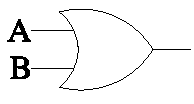
\includegraphics[width=2.5cm]{pictures/boole/or-ABC}}
%\end{center}
&
$A\lor B$
\\ \hline

Ja &
Ja-portti antaa jännitteen vain silloin, kun molemmissa sisäänmenoissa on jännite. &

%\begin{center}
\raisebox{-.5\height}{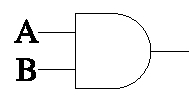
\includegraphics[width=2.5cm]{pictures/boole/and-ABC}}
%\end{center}
&
$A\land B$
\\ \hline

Ei &
Ei-portti antaa jännitteen silloin, kun sisäänmenossa ei ole jännitettä, ja kääntäen. &
%\begin{center}
\raisebox{-.5\height}{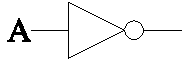
\includegraphics[width=2.5cm]{pictures/boole/not-ABC}}
%\end{center}
&
$\lnot A$
\\ \hline

\end{tabular}

\end{center}

\normalsize

%\newpage

\bigskip

Esimerkiksi looginen piiri

\medskip

\begin{center}
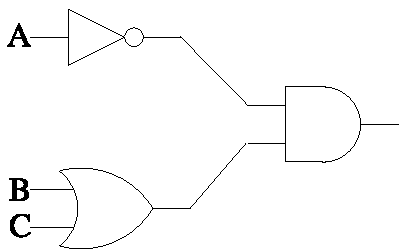
\includegraphics[width=3.5cm]{pictures/boole/boolesim-ABC}
\end{center}

\medskip
\noindent
koostuu kolmesta loogisesta portista ja vastaa
lausetta \mbox{$\lnot A\land (B \lor C)$}. %Muutettu alkuperäisestä, virhe joko tekstissä tai kuvassa.

%{\bf Tehtäviä}

%\begin{enumerate}
Muodosta seuraavia piirejä vastaavat lauseet.
    \begin{alakohdat}
        \alakohta{\begin{center}
		   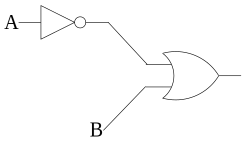
\includegraphics[width=3.5cm]{pictures/boole/boolt-a-ABC}
		   \end{center}}
	\alakohta{\begin{center}
		   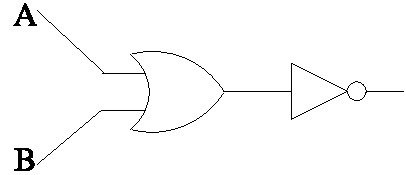
\includegraphics[width=3.5cm]{pictures/boole/boolt-b-ABC}
		   \end{center}}
        \alakohta{\begin{center}
		   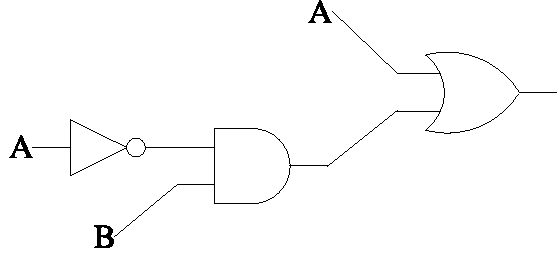
\includegraphics[width=4cm]{pictures/boole/boolt-c-ABC}
		   \end{center}}
        \alakohta{\begin{center}
		   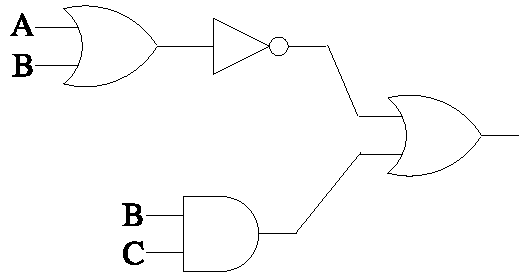
\includegraphics[width=4.5cm]{pictures/boole/boolt-d-ABC}
		   \end{center}}
    \end{alakohdat}

    \begin{vastaus}
        \begin{alakohdat}
            \alakohta{$\lnot A\lor B$}
            \alakohta{$\lnot(A\lor B)$}
            \alakohta{$A\lor (\lnot A \land B)$}
            \alakohta{$\lnot(A\lor B)\lor(B\land C)$}
        \end{alakohdat}
    \end{vastaus}
    
\end{tehtava}

\begin{tehtava}
    Piirrä lausetta
    \begin{alakohdat}
        \alakohta{$\lnot A \land B$}
        \alakohta{$A\lor \lnot (B\land C)$}
        \alakohta{$(A\land B)\lor (\lnot A \land C)$
vastaava looginen piiri.}
    \end{alakohdat}

    \begin{vastaus}
        \begin{alakohdat}
            \alakohta{KUVA!!!!!!!!!!} %Kuva puuttuu
            \alakohta{KUVA!!!!!!!!!!} %Kuva puuttuu
            \alakohta{KUVA!!!!!!!!!!} %Kuva puuttuu
        \end{alakohdat}
    \end{vastaus}
    
\end{tehtava}
%Luku 2 Kotitehtävät, Vastausten tekijä Valtteri Vistiaho 9.11.2013
\begin{tehtava}
    Kirjoita lauseen negaatio.
    \begin{alakohdat}
        \alakohta{$100 > 101$.}
        \alakohta{Lompakossani on rahaa korkeintaan 10 euroa.}
        \alakohta{Kaikki ryhmämme opiskelijat ovat Facebookissa.}
        \alakohta{Koulussamme on täsmälleen kaksi vasenkätistä opettajaa.}
        \alakohta{En opiskele latinaa enkä kreikkaa.}
        \alakohta{Maarit pitää lumilautailusta tai käsitöistä muttei molemmista.}
    \end{alakohdat}

    \begin{vastaus}
        \begin{alakohdat}
            \alakohta{$100\leq101$}
            \alakohta{Lompakossani on rahaa enemmän kuin 10 euroa.}
            \alakohta{Kaikki ryhmämme opiskelijat eivät ole Facebookissa.}
            \alakohta{Koulussamme on enemmän tai vähemmän kuin kaksi vasenkätistä opettajaa.}
            \alakohta{Opiskelen latinaa tai kreikkaa.}
            \alakohta{Maarit pitää lumilautailusta ja käsitöistä tai Maarit ei pidä lumilautailusta eikä käsitöistä. ?????????} %En ole täysin varma vastauksesta
        \end{alakohdat}
    \end{vastaus}
    
\end{tehtava}

\begin{tehtava}
    Olkoot lauseet $A$: ''puutarhan portti on auki'', $B$: ''ruusut kukkivat'' ja $C$: ''menen puutarhaan''. Kirjoita suomen kielellä lauseet
    \begin{alakohdat}
        \alakohta{$\lnot A$,}
        \alakohta{$B\land C$,}
        \alakohta{$A\lor B$,}
        \alakohta{$\lnot B \land \lnot C$,}
        \alakohta{$\lnot(A\land B)$,}
        \alakohta{ $A \lor \lnot B$ ja}
        \alakohta{$(A \land C) \lor (\lnot B \land C)$.}
    \end{alakohdat}

    \begin{vastaus}
        \begin{alakohdat}
            \alakohta{Puutarhan portti on kiinni.}
            \alakohta{Ruusut kukkivat ja menen puutarhaan.}
            \alakohta{Puutarhan portti on auki tai ruusut kukkivat.}
            \alakohta{Ruusut eivät kuki enkä mene puutarhaan.}
            \alakohta{Ei ole totta, että puutarhan portti on auki ja ruusut kukkivat.}
            \alakohta{Puutarhan portti on auki tai ruusut eivät kuki.}
            \alakohta{Puutarhan portti on auki ja menen puutarhaan, tai ruusut eivät kuki ja menen puutarhaan.}
        \end{alakohdat}
    \end{vastaus}
    
\end{tehtava}

\begin{tehtava}
    Formalisoi lause.
    \begin{alakohdat}
        \alakohta{Kaino ei ole vanha ja Kaino on mies.}
        \alakohta{Kaino on vanha tai Kaino ei ole mies.}
        \alakohta{Kaino ei ole vanha mies. }
        \alakohta{Kaino ei ole vanha eikä hän ole mies.}
    \end{alakohdat}

    \begin{vastaus}
    Olkoot $A$: ''Kaino on vanha.'' ja $B$: ''Kaino on mies.''
        \begin{alakohdat}
            \alakohta{$\lnot A\land B$}
            \alakohta{$A\lor \lnot B$}
            \alakohta{$\lnot(A\land B)$}
            \alakohta{$\lnot A\land \lnot B$}
        \end{alakohdat}
    \end{vastaus}
    
\end{tehtava}

\begin{tehtava}
    Formalisoi lause.
    \begin{alakohdat}
        \alakohta{Amadeus kuuntelee klassista tai Klaus kuuntelee jazzia.}
        \alakohta{Amadeus ei kuuntele klassista, mutta Klaus kuuntelee jazzia.}
        \alakohta{Amadeus kuuntelee klassista, mutta Klaus ei kuuntele jazzia, tai sitten Hassinen kuuntelee progea.}
        \alakohta{Ei ole niin, että Amadeus kuuntelisi klassista, Klaus jazzia ja Hassinen progea.}
    \end{alakohdat}

    \begin{vastaus}
    Olkoot $A$: ''Amadeus kuuntelee klassista.'', $B$: ''Klaus kuuntelee jazzia.'' ja $C$: ''Hassinen kuuntelee progea.''
        \begin{alakohdat}
            \alakohta{$A\lor B$}
            \alakohta{$\lnot A\land B$}
            \alakohta{$(A\land \lnot B)\lor C$}
            \alakohta{$\lnot (A\land B\land C)$}
        \end{alakohdat}
    \end{vastaus}
    
\end{tehtava}

\begin{tehtava}
    
    \begin{alakohdat}
        \alakohta{Laadi totuustaulu lauseille $A\land \lnot A$ ja $A\lor \lnot A$.}
        \alakohta{Keksi atomilause $A$ ja ilmaise kohdan a) lauseet suomen kielellä.}
    \end{alakohdat}

    \begin{vastaus}
        \begin{alakohdat}
            \alakohta{
            \begin{center}
		    \begin{tabular}{|c|c|c|c|}\hline
		    $A$ & $\lnot A$ & $A\land \lnot A$ & $A\lor \lnot A$\\ \hline
		    $1$ & $0$ & $0$ & $1$  \\ %\hline
		    $1$ & $0$ & $0$ & $1$ \\
		    $0$ & $1$ & $0$ & $1$ \\
		    $0$ & $1$ & $0$ & $1$ \\ \hline
\end{tabular}
\end{center}}
            \alakohta{Ulkona sataa ja ulkona ei sada. \\ 
            Ulkona sataa tai ulkona ei sada.}
        \end{alakohdat}
    \end{vastaus}
    
\end{tehtava}

\begin{tehtava}
    Laadi totuustaulu lauseille
    \begin{alakohdat}
        \alakohta{$\lnot(A\lor B)$,}
        \alakohta{$\lnot A\land B$,}
        \alakohta{$(\lnot A\lor B)\land (A\lor \lnot B)$. \\ 
        Millä atomilauseiden $A$ ja  $B$ totuusarvojen yhdistelmillä lauseet ovat tosia?} 
    \end{alakohdat}

    \begin{vastaus}
        \begin{alakohdat}
            \alakohta{\begin{center}
		    \begin{tabular}{|c|c|c|c|}\hline
		    $A$ & $B$ & $A\lor B$ & $\lnot(A\lor B)$\\ \hline
		    $1$ & $1$ & $1$ & $0$ \\ %\hline
		    $1$ & $0$ & $0$ & $1$ \\
		    $0$ & $1$ & $1$ & $0$ \\
		    $0$ & $0$ & $1$ & $0$ \\ \hline \\
		    Lause on tosi, kun $A$ on tosi ja $B$ epätosi.
\end{tabular}
\end{center}}
            \alakohta{\begin{center}
		    \begin{tabular}{|c|c|c|c|}\hline
		    $A$ & $B$ & $\lnot A$ & $\lnot A\land B$ \\ \hline
		    $1$ & $1$ & $0$ & $0$  \\ %\hline
		    $1$ & $0$ & $0$ & $0$ \\
		    $0$ & $1$ & $1$ & $1$ \\
		    $0$ & $0$ & $1$ & $0$ \\ \hline \\
		    Lause on tosi, kun $A$ on epätosi ja $B$ tosi.
\end{tabular}
\end{center}}
            \alakohta{\begin{center}
		    \begin{tabular}{|c|c|c|c|c|c|c|}\hline
		    $A$ & $B$ & $\lnot A$ & $\lnot B$ & $(\lnot A\lor B)$ & $(A\lor \lnot B)$ & $(\lnot A\lor B)\land (A\lor \lnot B)$ \\ \hline
		    $1$ & $1$ & $0$ & $0$ & $1$ & $1$ & $1$ \\ %\hline
		    $1$ & $0$ & $0$ & $1$ & $0$ & $1$ & $0$ \\
		    $0$ & $1$ & $1$ & $0$ & $1$ & $0$ & $0$ \\
		    $0$ & $0$ & $1$ & $1$ & $1$ & $1$ & $1$ \\ \hline \\
		    Lause on tosi, kun $A$ ja $B$ ovat tosia.
\end{tabular}
\end{center}}
        \end{alakohdat}
    \end{vastaus}
    
\end{tehtava}

\begin{tehtava}
    
    \begin{alakohdat}
        \alakohta{Laadi totuustaulu lauseelle $A\lor (B\land C)$.}
        \alakohta{Laadi totuustaulu lauseelle $(A\lor B)\land C$.}
        \alakohta{Vertaa kohtien a) ja b) lauseiden totuusarvoja. Mitä voit päätellä?}
    \end{alakohdat}

    \begin{vastaus}
        \begin{alakohdat}
            \alakohta{
            \begin{center}
		    \begin{tabular}{|c|c|c|c|}\hline
		    $A$ & $B$ & $C$ & $A\lor (B\land C)$\\ \hline
		    $1$ & $1$ & $1$ & $1$ \\ %\hline
		    $1$ & $1$ & $0$ & $1$ \\
		    $1$ & $0$ & $1$ & $1$ \\
		    $1$ & $0$ & $0$ & $1$ \\
		    $0$ & $1$ & $1$ & $1$ \\
		    $0$ & $0$ & $1$ & $0$ \\
		    $0$ & $1$ & $0$ & $0$ \\
		    $0$ & $0$ & $0$ & $0$ \\ \hline
\end{tabular}
\end{center}}
            \alakohta{
            \begin{center}
		    \begin{tabular}{|c|c|c|c|}\hline
		    $A$ & $B$ & $C$ & $(A\lor B)\land C$\\ \hline
		    $1$ & $1$ & $1$ & $1$ \\ %\hline
		    $1$ & $1$ & $0$ & $0$ \\
		    $1$ & $0$ & $1$ & $1$ \\
		    $1$ & $0$ & $0$ & $0$ \\
		    $0$ & $1$ & $1$ & $1$ \\
		    $0$ & $0$ & $1$ & $0$ \\
		    $0$ & $1$ & $0$ & $0$ \\
		    $0$ & $0$ & $0$ & $0$ \\ \hline
\end{tabular}
\end{center}}
            \alakohta{Sulkujen paikka on merkitsevä, ???????????????????} %En tiedä, mitä tehtävän tekijä tässä ajaa takaa.
        \end{alakohdat}
    \end{vastaus}
    
\end{tehtava}

\begin{tehtava}
    
    \begin{alakohdat}
        \alakohta{}
        \alakohta{}
        \alakohta{}
        \alakohta{}
    \end{alakohdat}

    \begin{vastaus}
        \begin{alakohdat}
            \alakohta{}
            \alakohta{}
            \alakohta{}
            \alakohta{}
        \end{alakohdat}
    \end{vastaus}
    
\end{tehtava}

\begin{tehtava}
    
    \begin{alakohdat}
        \alakohta{}
        \alakohta{}
        \alakohta{}
        \alakohta{}
    \end{alakohdat}

    \begin{vastaus}
        \begin{alakohdat}
            \alakohta{}
            \alakohta{}
            \alakohta{}
            \alakohta{}
        \end{alakohdat}
    \end{vastaus}
    
\end{tehtava}

\begin{tehtava}
    
    \begin{alakohdat}
        \alakohta{}
        \alakohta{}
        \alakohta{}
        \alakohta{}
    \end{alakohdat}

    \begin{vastaus}
        \begin{alakohdat}
            \alakohta{}
            \alakohta{}
            \alakohta{}
            \alakohta{}
        \end{alakohdat}
    \end{vastaus}
    
\end{tehtava}

\begin{tehtava}
    
    \begin{alakohdat}
        \alakohta{}
        \alakohta{}
        \alakohta{}
        \alakohta{}
    \end{alakohdat}

    \begin{vastaus}
        \begin{alakohdat}
            \alakohta{}
            \alakohta{}
            \alakohta{}
            \alakohta{}
        \end{alakohdat}
    \end{vastaus}
    
\end{tehtava}

\begin{tehtava}
    
    \begin{alakohdat}
        \alakohta{}
        \alakohta{}
        \alakohta{}
        \alakohta{}
    \end{alakohdat}

    \begin{vastaus}
        \begin{alakohdat}
            \alakohta{}
            \alakohta{}
            \alakohta{}
            \alakohta{}
        \end{alakohdat}
    \end{vastaus}
    
\end{tehtava}

\begin{tehtava}
    
    \begin{alakohdat}
        \alakohta{}
        \alakohta{}
        \alakohta{}
        \alakohta{}
    \end{alakohdat}

    \begin{vastaus}
        \begin{alakohdat}
            \alakohta{}
            \alakohta{}
            \alakohta{}
            \alakohta{}
        \end{alakohdat}
    \end{vastaus}
    
\end{tehtava}

\begin{tehtava}
    
    \begin{alakohdat}
        \alakohta{}
        \alakohta{}
        \alakohta{}
        \alakohta{}
    \end{alakohdat}

    \begin{vastaus}
        \begin{alakohdat}
            \alakohta{}
            \alakohta{}
            \alakohta{}
            \alakohta{}
        \end{alakohdat}
    \end{vastaus}
    
\end{tehtava}

\begin{tehtava}
    
    \begin{alakohdat}
        \alakohta{}
        \alakohta{}
        \alakohta{}
        \alakohta{}
    \end{alakohdat}

    \begin{vastaus}
        \begin{alakohdat}
            \alakohta{}
            \alakohta{}
            \alakohta{}
            \alakohta{}
        \end{alakohdat}
    \end{vastaus}
    
\end{tehtava}

\begin{tehtava}
    
    \begin{alakohdat}
        \alakohta{}
        \alakohta{}
        \alakohta{}
        \alakohta{}
    \end{alakohdat}

    \begin{vastaus}
        \begin{alakohdat}
            \alakohta{}
            \alakohta{}
            \alakohta{}
            \alakohta{}
        \end{alakohdat}
    \end{vastaus}
    
\end{tehtava}

\begin{tehtava}
    
    \begin{alakohdat}
        \alakohta{}
        \alakohta{}
        \alakohta{}
        \alakohta{}
    \end{alakohdat}

    \begin{vastaus}
        \begin{alakohdat}
            \alakohta{}
            \alakohta{}
            \alakohta{}
            \alakohta{}
        \end{alakohdat}
    \end{vastaus}
    
\end{tehtava}

\begin{tehtava}
    
    \begin{alakohdat}
        \alakohta{}
        \alakohta{}
        \alakohta{}
        \alakohta{}
    \end{alakohdat}

    \begin{vastaus}
        \begin{alakohdat}
            \alakohta{}
            \alakohta{}
            \alakohta{}
            \alakohta{}
        \end{alakohdat}
    \end{vastaus}
    
\end{tehtava}

\begin{tehtava}
    
    \begin{alakohdat}
        \alakohta{}
        \alakohta{}
        \alakohta{}
        \alakohta{}
    \end{alakohdat}

    \begin{vastaus}
        \begin{alakohdat}
            \alakohta{}
            \alakohta{}
            \alakohta{}
            \alakohta{}
        \end{alakohdat}
    \end{vastaus}
    
\end{tehtava}

%Harj.Tehtävät Luku 6

% \section{Suurin yhteinen tekijä ja Eukleideen algoritmi}
\begin{tehtava}
    Määritä lukujen suurin yhteinen tekijä.
    
    \begin{alakohdat}
        \alakohta{$15$ ja $20$}
        \alakohta{$9$ ja $36$}
        \alakohta{$4$ ja $7$}
    \end{alakohdat}

    \begin{vastaus}
        \begin{alakohdat}
            \alakohta{$5$}
            \alakohta{$9$}
            \alakohta{$1$}
        \end{alakohdat}
    \end{vastaus}
    
\end{tehtava}

\begin{tehtava}
    Määritä Eukleideen algoritmia käyttäen
    
    \begin{alakohdat}
        \alakohta{$\syt(184, 152)$}
        \alakohta{$\syt(227, 143)$.}
    \end{alakohdat}

    \begin{vastaus}
        \begin{alakohdat}
            \alakohta{$8$}
            \alakohta{$1$}
        \end{alakohdat}
    \end{vastaus}
    
\end{tehtava}

\begin{tehtava}
    Määritä Eukleideen algoritmia käyttäen
    
    \begin{alakohdat}
        \alakohta{$\syt(272, 1479)$}
        \alakohta{$\syt(4719, 18207)$.}
    \end{alakohdat}

    \begin{vastaus}
        \begin{alakohdat}
            \alakohta{$17$}
            \alakohta{$3$}
        \end{alakohdat}
    \end{vastaus}
    
\end{tehtava}

\begin{tehtava}
    Esitä murtoluku
    \begin{alakohdat}
        \alakohta{$\frac{143}{605}$}
        \alakohta{$\frac{5989}{30899}$}
    \end{alakohdat}
    supistetussa muodossa. Vihje: Määritä osoittajan ja nimittäjän suurin yhteinen tekijä.

    \begin{vastaus}
        \begin{alakohdat}
            \alakohta{$\frac{13}{55}$}
            \alakohta{$\frac{113}{583}$}
        \end{alakohdat}
    \end{vastaus}
    
\end{tehtava}

\begin{tehtava}
    % Tarkistettu (Topi Talvitie, 9.11.2013)
    Osoita, että murtoluku $\frac{8788}{13475}$ ei supistu.
\end{tehtava}

\begin{tehtava}
    Leirille osallistui 780 tyttöä ja 612 poikaa. Osallistujat jaettiin keskenään yhtä suuriin ryhmiin siten, että kussakin ryhmässä oli vain tyttöjä tai poikia. Mikä oli suurin mahdollinen ryhmäkoko?
    
    \begin{vastaus}
        12
    \end{vastaus}
    
\end{tehtava}

\begin{tehtava}
    Määritä lukujen $188000100$ ja $188$ suurin yhteinen tekijä.

    \begin{vastaus}
        $4$
    \end{vastaus}
    
\end{tehtava}

\begin{tehtava}
    Olkoon $a$ positiivinen kokonaisluku. Määritä
    \begin{alakohdat}
        \alakohta{$\syt(a, a)$}
        \alakohta{$\syt(a, 1)$}
        \alakohta{$\syt(a^2, a)$}
        \alakohta{$\syt((a+1)!, a!)$.}
    \end{alakohdat}
    Merkintä $a!$ tarkoittaa luvun $a$ \termi{kertoma}{kertomaa}. Se on tulo $a! = a \cdot (a-1) \cdot (a-2) \cdot \ldots \cdot 3 \cdot 2 \cdot 1$.

    \begin{vastaus}
        \begin{alakohdat}
            \alakohta{$a$}
            \alakohta{$1$}
            \alakohta{$a$}
            \alakohta{$a!$}
        \end{alakohdat}
    \end{vastaus}
    
\end{tehtava}

\begin{tehtava}
    % Tarkistettu (Topi Talvitie, 9.11.2013)
    Olkoon $n$ positiivinen kokonaisluku. Osoita Eukleideen algoritmia käyttäen, että $\syt(n+1, n)=1$.
\end{tehtava}

\begin{tehtava}
    Olkoon $n$ positiivinen kokonaisluku. Määritä lukujen $n^2 + 2n$ ja $n + 1$ suurin yhteinen tekijä.
    
    \begin{vastaus}
        1
    \end{vastaus}
    
\end{tehtava}

\begin{tehtava}
    % Tarkistettu (Topi Talvitie, 9.11.2013)
    Olkoon $n$ positiivinen kokonaisluku. Osoita, että
    \[\syt(3^{n+1} + 10, 3^n + 2)=1.\]
\end{tehtava}

% \subsection*{Kotitehtäviä}
\begin{tehtava}
    Määritä lukujen suurin yhteinen tekijä.
    
    \begin{alakohdat}
        \alakohta{$63$ ja $7$}
        \alakohta{$64$ ja $33$}
        \alakohta{$45$ ja $60$}
    \end{alakohdat}

    \begin{vastaus}
        \begin{alakohdat}
            \alakohta{$7$}
            \alakohta{$1$}
            \alakohta{$15$}
        \end{alakohdat}
    \end{vastaus}
    
\end{tehtava}

\begin{tehtava}
    Määritä Eukleideen algoritmia käyttäen
    
    \begin{alakohdat}
        \alakohta{$\syt(657, 306)$}
        \alakohta{$\syt(2197, 4641)$}
        \alakohta{$\syt(15787, 4111)$.}
    \end{alakohdat}

    \begin{vastaus}
        \begin{alakohdat}
            \alakohta{$9$}
            \alakohta{$13$}
            \alakohta{$1$}
        \end{alakohdat}
    \end{vastaus}
    
\end{tehtava}

\begin{tehtava}
    Esitä murtoluku
    \begin{alakohdat}
        \alakohta{$\frac{182}{299}$}
        \alakohta{$\frac{7697}{32041}$}
    \end{alakohdat}
    supistetussa muodossa.

    \begin{vastaus}
        \begin{alakohdat}
            \alakohta{$\frac{14}{23}$}
            \alakohta{$\frac{43}{179}$}
        \end{alakohdat}
    \end{vastaus}
    
\end{tehtava}

\begin{tehtava}
    Leipomo suljettiin remontin ajaksi. Ennen sulkemista laskettiin, että leipomon varastossa oli 4896 vehnäsämpylää ja 1408 grahamsämpylää. Sämpylät pakattiin kuljetusta varten keskenään samankokoisiin pusseihin siten, että kuhunkin pussiin tuli vain vehnä- tai grahamsämpylöitä. Mikä oli suurin mahdollinen pussikoko? Oletetaan, että vehnäsämpylä oli samankokoinen kuin grahamsämpylä ja että yksikään pussi ei jäänyt vajaaksi.

    \begin{vastaus}
        $32$
    \end{vastaus}
    
\end{tehtava}

\begin{tehtava}
    Määritä lukujen $468468468108$ ja $234$ suurin yhteinen tekijä.
    
    \begin{vastaus}
        $18$
    \end{vastaus}
    
\end{tehtava}

\begin{tehtava}
    Olkoot $a$, $b$ ja $c$ positiivisia kokonaislukuja. Lukujen $a$, $b$ ja $c$ suurin yhteinen tekijä eli $\syt(a, b, c)$ voidaan määrittää siten, että ensin määritetään kahden luvun suurin yhteinen tekijä ja sitten tämän ja kolmannen luvun suurin yhteinen tekijä. Määritä
    
    \begin{alakohdat}
        \alakohta{$\syt(15, 30, 40)$}
        \alakohta{$\syt(6, 9, 11)$}
        \alakohta{$\syt(171, 456, 665)$.}
    \end{alakohdat}

    \begin{vastaus}
        \begin{alakohdat}
            \alakohta{$5$}
            \alakohta{$1$}
            \alakohta{$19$}
        \end{alakohdat}
    \end{vastaus}
    
\end{tehtava}

\begin{tehtava}
    Olkoot $a$ ja $b$ positiivisia kokonaislukuja ja $\syt(a, b)=9$. Voiko tällöin yhtälö $a + b = 186$ olla tosi?
    
    \begin{vastaus}
        Ei voi.
    \end{vastaus}
    
\end{tehtava}

\begin{tehtava}
    Olkoon $n$ positiivinen kokonaisluku. Tutki, mitä arvoja $\syt(n+4, n)$ voi saada.
    
    \begin{vastaus}
        $1$, $2$ ja $4$.
    \end{vastaus}
    
\end{tehtava}

\begin{tehtava}
    Olkoon $n$ positiivinen kokonaisluku. Määritä lukujen $n^2 + 3n$ ja $n + 2$ suurin yhteinen tekijä.
    
    \begin{vastaus}
        Jos $n$ on parillinen, $\syt(n^2 + 3n, n + 2) = 2$, muuten $\syt(n^2 + 3n, n + 2) = 1$.
    \end{vastaus}
    
\end{tehtava}

\begin{tehtava}
    % Tarkistettu (Topi Talvitie, 9.11.2013)
    Olkoot $a$ ja $b$ positiivisia kokonaislukuja. Osoita, että $\syt(a, b)$ on jaollinen kaikilla lukujen $a$ ja $b$ yhteisillä tekijöillä.
\end{tehtava}

